%%%%%%%%%%%%%%%%%%%%%%%%%%%%%%%%%%%%%%%%%%%%%%%%%%%%%%%%%%%%%%%%%%
\section{Lessons for FSI solver developers}
\label{app:lessons}
%%%%%%%%%%%%%%%%%%%%%%%%%%%%%%%%%%%%%%%%%%%%%%%%%%%%%%%%%%%%%%%%%%
% Sources: solids4foam_learnings.md (register entries 1-18), the defect
% table of Section 6 (sec:defects), Sections 5.1.3, 5.3.1 and 5.3.2, and
% paper-data/r1_audit/ for the coupling-test audit.

This appendix collects the issues that the verification campaign revealed in the code under test, its set-ups and the benchmark definitions.
Each is stated generically, with solids4foam as the example, together with the evidence that revealed it and how it was resolved or what remains open.
None was found by comparison with a published benchmark value; the defects proper are also listed in Table~\ref{tab:defects}.

\paragraph{Aliasing in field algebra under optimisation.}
In the 3-D pressure-pulse tube (Section~\ref{sec:3dtube}) two platforms gave deterministic results that differed by $1.5$--$3\%$ in one QoI while the others agreed to $0.1$--$0.2\%$.
The wall viscous force was formed as an inner product of two temporary fields; OpenFOAM's field algebra writes such a product into the storage of a temporary operand while its loops access result and operands through \texttt{\_\_restrict\_\_} pointers, so at \texttt{-O3} one component was formed from already overwritten values, whereas \texttt{-O2} builds were correct.
The site and about 15 others with the same mechanism were corrected.
The general lesson is that the compiled executable is the code under test: the compiler and optimisation level belong in the verification record, and a replicate on a second build or platform is a cheap check that no refinement study on one platform replaces.

\paragraph{Scale-dependent tolerances in interpolation weights.}
After the correction above, the first remaining divergence between the platforms, a broken symmetry of the quarter tube and a dependence on the domain decomposition led to the solid-to-fluid point transfer.
Its barycentric weights fell back to the degenerate values $(1/3, 1/3, 1/3)$ when the squared triangle area fell below a fixed absolute threshold, which every interface triangle of levels 2 and 3 did but none of level 1; the interpolation operator therefore changed with refinement, and the mesh study compared different operators.
Scale-invariant weights resolved it.
Any absolute geometric tolerance in a transfer or search operator should be suspected when an observed order changes between levels; symmetry and decomposition-invariance checks expose it at little cost.

\paragraph{Coupling convergence tests.}
A test that accepts a step when the smaller of two residual measures, one relative to the largest residual of the step ($r_1$) and one relative to the total interface displacement ($r_2$), is below the tolerance does not bound the reduction of the interface residual within the step.
An audit of the solver logs (\texttt{paper-data/r1\_audit/}) found steps accepted with $r_1$ above the tolerance in every benchmark audited: in $21$--$36\%$ of the steps of the ring added-mass problem and about $31\%$ of those of the 3-D pressure-pulse tube ($r_1$ at most $12$ times the tolerance); in almost every step of the FSI2 study, of the uniform FSI3 family (median $r_1$ about ten times the tolerance) and of the Robin--Neumann runs of the Womersley tube ($r_1 \leq 60$ times the tolerance), but not in the IQN-ILS run of the Womersley tube; and, worst, in steady problems, where an FSI1 run accepted $r_1 = 0.72$ and the flexible-bottom cavity accepted pseudo-time steps after a single iteration with $r_1 = 1$, i.e.\ with no reduction of the interface mismatch.
For the collapsible channel, FSI2 and the Mok lid-driven cavity, runs with the same set-up and coupling settings were audited in place of the reported studies, whose logs were not kept.
In the Hessenthaler flap the accepted steps produced a slow drift larger than the spatial differences under study (Section~\ref{sec:iterative_errors}).
No step of the strict-test FSI3 runs ($\approx8.8\times10^{4}$ coupled steps on three levels) was accepted with $r_1$ above the tolerance.
The remedy is to require every measure to meet the tolerance and to record the residuals at acceptance.
A purely relative measure has its own limitation: $r_1$ is normalised by the largest residual of the step, so at a true steady state the residual is at round-off from the first iteration, $r_1$ cannot fall below the tolerance, and every step runs to the iteration limit with a false warning, at four to six times the cost; an absolute floor on $r_1$ is the obvious remedy and is not yet implemented.

\paragraph{Boundary non-orthogonal corrections that vanish silently.}
Several boundary conditions, including the moving-wall and interface velocity conditions of the fluid, build their non-orthogonal correction from the tangential part of the boundary delta vector.
On the OpenCFD releases used here that vector is purely normal on non-coupled patches, so the correction is identically zero, while on another OpenFOAM fork it is not.
The omission was found with the tilting-interface variant of the manufactured solution, whose orders separate the effect of boundary non-orthogonality (Section~\ref{sec:mms_fsi}).
On a moving wall it leaves a viscous traction error of about $\nu\tan\theta\,|\partial\bb{v}/\partial\tau|$ that does not vanish under refinement at a fixed non-orthogonality angle $\theta$; it is zero at a steady state, where the wall velocity does not vary along the wall.
Its effect on the transient partitioned results is small (Section~\ref{sec:fluid_solver}); on the manufactured solution, a velocity condition of the quasi-monolithic fluid that does correct the viscous boundary gradient changed the errors by less than $1\%$.
The limitation is not specific to FSI: on the releases concerned, any calculation that uses these velocity conditions on a wall whose velocity varies along it and whose adjacent cells are non-orthogonal, for example a moving or deforming wall in a pure CFD problem, carries the same error.
A unit test that a boundary correction is non-zero on a skewed patch would have caught it.

\paragraph{Interpolation of the continuity flux.}
In the flexible-bottom cavity (Section~\ref{sec:cavity}), four levels gave a steady force limit with a GCI of $0.02\%$ that lay $0.05\%$ from three other solutions, a fully independent SU2--CalculiX solution, a FEniCSx solution and a quasi-monolithic solution of the same code family, which agree with one another.
The face flux of the continuity equation was interpolated with plain linear interpolation, the default, although the velocity interpolation of the set-up was skew-corrected; near the clamped ends of the plate the deformed cells are strongly skewed, and the resulting error converges so slowly that the sequence looks converged.
With a skew-corrected continuity flux the limit agrees with all three to within $0.016\%$.
On a moving or deforming mesh, every interpolated flux should be checked for skew correction, not only those named in the set-up; and a small GCI from one code is not evidence that the limit is correct.

\paragraph{A steady state that depends on the pseudo-time step.}
A steady solution reached by pseudo-time stepping of a segregated solver with momentum interpolation depends on the pseudo-time step, since the coefficient of the pressure--velocity coupling term does.
In the flexible-bottom cavity the force changed by $0.18\%$ on level 1 when $\Delta t$ was reduced eightfold, but only by $0.03\%$ and $0.001\%$ on levels 2 and 3.
A steady study should state $\Delta t$ per level and repeat one level at a second $\Delta t$; when $\Delta t$ is scaled with $h$, this dependence is mixed into the mesh convergence.

\paragraph{Path-dependent mesh motion.}
In Turek--Hron FSI3 the uniform block-structured family of Section~\ref{sec:fsi23}, computed with a Laplacian of the mesh velocity, a zero-gradient wall pressure and gradient-limited linear-upwind convection, gave displacements that converge monotonically at an observed order of $0.9$--$1.1$ ($u_y$ amplitude $29.85$, $34.18$ and $36.23\,\mathrm{mm}$ on 1x, 2x and 4x, against $34.99\,\mathrm{mm}$ for Featflow).
The 2x level agreed with Featflow to $2$--$3\%$, but this was a crossing: at 4x the displacements lay beyond the reference ($u_y$ amplitude $+3.5\%$, $u_x$ mean $-7.1\%$) and were still moving away, and the two-level apparent orders against Featflow from 1x and 2x ($2.6$--$3.8$) were artefacts of the crossing.
Isolating the components located the cause.
The solid alone, on the FSI3 flag (the CSM2 and CSM3 tests of~\citet{Turek2006}) refined to 8x, approaches second order (observed orders $1.4$--$1.6$ on 1x--4x, $1.8$--$1.9$ on 2x--8x), and refining only the solid inside FSI3 changes the $u_y$ amplitude by $+0.33\%$, about $5\%$ of the coupled 2x$\to$4x change, although it changes the lift and drag amplitudes by $-12.3\%$ and $-5.5\%$.
With the flag held rigid (CFD3) the drag mean and lift amplitude converge monotonically to within $0.16\%$ and $0.05\%$ of the Featflow values.
The aliasing and interpolation-weight defects above have no effect on this two-dimensional case: runs with and without their corrections are identical to every written digit.
With the coupled 2x interface motion prescribed on fluid-only meshes, the generalised fluid force on the flag in phase with its displacement, $Q_\mathrm{in}$, converged at first order ($50.3$, $72.2$ and $81.0\,\mathrm{N/m}$; observed order 1.3), and changing one fluid treatment at a time moved $Q_\mathrm{in}$ but left its order at $1.1$--$1.3$ for the treatments run on three levels (wall pressure, gradient scheme), with the same first-order-like behaviour on two levels for the wall velocity condition and the mesh-motion diffusivity; the regions near the free-end corners carry only $22\%$ of its change.
The cause is the mesh motion: a Laplacian of the mesh velocity is path dependent, so under periodic motion the interior mesh drifts from cycle to cycle, $Q_\mathrm{in}$ rose without settling ($+0.3\,\mathrm{N/m}$ per second at 1x), and the levels were compared after different elapsed times; a Laplacian of the mesh displacement with the same diffusivity holds $Q_\mathrm{in}$ steady to $\pm0.03\,\mathrm{N/m}$.
With a mesh motion that depends only on the current interface position and an acceleration-consistent wall pressure (below), the first-order displacement sequence does not recur (Section~\ref{sec:fsi23}).
For periodic problems the mesh motion should be a function of the current interface position, not of its history, and a two-level agreement with a reference should not be read as convergence.

\paragraph{Wall pressure and wall velocity conditions.}
A zero normal pressure gradient on an accelerating wall omits the term $-\rho_F\,\bb{n}\cdot\bb{a}$ of the normal momentum equation and gives an $O(h)$ wall-pressure error; it contributed to the first-order FSI3 sequence above.
A flux-based pressure condition, applied on a wall where the velocity is prescribed, silently reduces to a zero gradient, as an independent preCICE solution of FSI3 showed when its two variants agreed to $2\times10^{-5}$.
An acceleration-consistent condition is used here (Section~\ref{sec:fluid_solver}); its viscous term is still omitted.
Separately, the wall-normal derivative of the normal velocity in the moving-wall condition was inconsistent with continuity. Correcting it changes, on a block-structured FSI3 mesh of 47\,056 fluid cells, the $u_x$ mean and amplitude by $-3.1\%$, the $u_y$ amplitude by $-1.5\%$, the drag amplitude by $-3.8\%$ and the lift amplitude by $-2.2\%$, all towards the reference, and the frequency and drag mean by at most $0.2\%$; it changes the ring added-mass problem and the collapsible channel by less than $10^{-3}$ relative, the Womersley tube by about $10^{-4}$ of the exact values, and FSI1 and FSI2 (1x) by at most $0.4\%$.
The wall conditions of the fluid on a moving interface are part of the coupled discretisation and deserve their own order tests.

\paragraph{Errors that only an exact finite-deformation solution exposes.}
The manufactured solution (Section~\ref{sec:mms_fsi}) revealed errors that the linear exact problems could not. They are described here for the partitioned results of Table~\ref{tab:mms_fsi} \hl{[pending: revise after the fluid/solid fixes]}.

\emph{Solid.}
Two errors of the total Lagrangian solid, both identified in runs of the solid alone driven by the exact interface traction, account for the partitioned solid results.
At $t = 0.2$ the partitioned solid and interface displacements converge at first order ($0.85$--$1.08$) on every pair of levels, with almost the same errors for the two couplings, whereas the quasi-monolithic solid displacement converges at $2.02$--$2.16$ (\texttt{paper-data/mms\_fsi/order\_tables/}).
This is explained by a start-up error of the displacement-form solid, which is first order in time when the motion starts from rest with a non-zero acceleration, as it does here: the time factors~\eqref{eq:mms_r} vanish with their first derivatives at $t = 0$, but not with their second.
In the solid alone this error is about $8.6\times10^{-5}$ at $t = 0.1$ on every mesh, with $\Delta t = 6.25\times10^{-4}$, and falls fourfold when $\Delta t$ is divided by four; scaled linearly to the time steps of Table~\ref{tab:mms_fsi}, it is of the size of the partitioned displacement errors at $t = 0.2$ ($2.6\times10^{-3}$ to $3.9\times10^{-4}$ from $n = 16$ to $128$ with Aitken).
With $\Delta t \propto h$, it appears as a first-order spatial error in the combined study; the quasi-monolithic coupling uses the velocity form of the solid, which does not show it.
The drop of the order to $0.7$--$0.8$ from $n = 64$ to $128$ at $t = 0.4$ matches a second, spatial error that both total Lagrangian solids share.
The deformed area of a traction boundary, $J|\bb{F}^{-T}\bb{N}|$, is evaluated with the deformation gradient of the adjacent cell, half a cell from the face, so the traction data of the solid carry an $O(h)$ error; it scales with the traction and with the normal derivative of the tangential stretch, both of which grow strongly after $t \approx 0.2$, so the order is lost on the finest meshes first.
For the displacement form, successive-mesh differences of the solid alone at $t = 0.4$ converge at $2.23$ and $1.53$; evaluating the tangential part of the boundary deformation gradient from a surface gradient over the face restores $2.30$ and $2.19$.

\emph{Fluid.}
The partitioned fluid converges at first order in pressure, and the largest velocity and pressure errors lie at the outlet; on $n = 128$ at $t = 0.4$ the pressure error is largest in the cells next to the outlet, positive in its lower half and negative in its upper half, with a maximum of $7.1\times10^{-2}$ against $3.1\times10^{-3}$ for the quasi-monolithic coupling (Fig.~\ref{fig:mms_fsi}).
The velocity maximum norm converges at orders of only $0.4$--$1.2$ and the pressure maximum norm at $0.5$--$0.7$.
The errors belong to the fluid, not to the coupling: the partitioned fluid alone, with the mesh following the exact interface motion and the moving-wall velocity on the interface, reproduces the coupled Aitken errors to within $3\%$ in pressure and $6\%$ in velocity, with the same orders, whereas the quasi-monolithic fluid alone converges at second order (pressure $2.03$, $2.02$; velocity $1.81$, $1.87$; full variant, $t = 0.4$, $n = 16$ to $64$; \texttt{paper-data/mms\_fsi/results/}).
The velocity error at the corner of the outlet and the bottom wall comes from the outlet condition, a prescribed velocity gradient with a prescribed pressure: with the exact velocity prescribed at the outlet instead, the velocity maximum norm converges at $1.6$--$1.9$ instead of $0.4$--$0.8$, the coupled velocity at second order ($2.03$, $2.05$), and the coupled pressure error falls by a factor of $2.9$ on $n = 64$, to orders $1.40$ and $1.36$.
The time-derivative correction of the momentum-interpolated face flux makes the pressure error grow as $\Delta t$ falls on a fixed mesh (on $n = 32$ from $3.4\times10^{-2}$ at $\Delta t = 0.02$ to $5.7\times10^{-2}$ at $\Delta t = 0.0025$), so with $\Delta t \propto h$ it adds a part that does not converge; it is the partitioned counterpart, of opposite sign, of the $\Delta t$-dependent stabilisation coefficient of the quasi-monolithic fluid.
Without this correction and at small $\Delta t$ ($6.25\times10^{-4}$) the interior pressure converges at second order ($1.9$ for $x < 1.5$, $2.0$ for $x < 1.0$); the first-order L2 error that remains is a thin layer in the outlet cells, with its maximum at $x = 1.984$, and with $\Delta t \propto h$ the interior error is then mostly a uniform offset of the pressure level that halves with $\Delta t$ (mean $-1.4\times10^{-2}$ to $-6.1\times10^{-3}$), i.e.\ first order in time.
Boundary non-orthogonality (the flat variant gives the same orders), the gradient scheme (least squares instead of Gauss linear), the interface pressure condition (a moving-wall pressure condition, also at small $\Delta t$), the interface velocity condition (the exact interface velocity), and, in the coupled calculation, a skew-corrected interpolation of the face flux in the pressure equation and the exact pressure gradient on the bottom wall each leave the errors unchanged; the remaining candidates for the outlet layer and the pressure-level offset are the pressure--velocity splitting with a single outer corrector on the moving mesh, the mass balance between the fixed-pressure outlet and the flux-consistent inlet, and the mesh flux.

\begin{figure}[htbp]
	\centering
	% Source: paper-data/mms_fsi/figure/mms_fsi_figure.py with the runs
	% mms-pfv/base/aitken-n128 and mms-fsi/case/runs/qm-full/n128 at time 0.4
	% (see paper-data/mms_fsi/README.md); fields were written only at t = 0.4.
	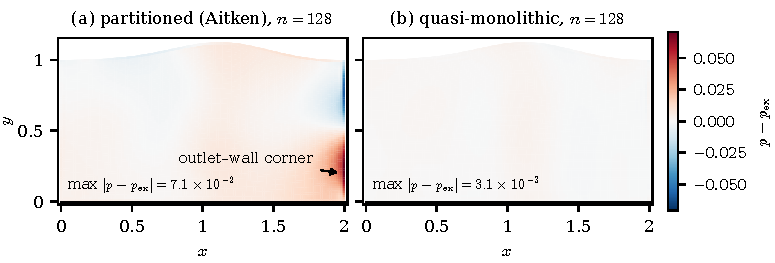
\includegraphics{figures/mms_fsi_pressure_error}
	\caption{Manufactured FSI solution: fluid pressure error $p - p_\mathrm{ex}$ at the cell centres at $t = 0.4$, full variant, $n = 128$ ($128\times64$ fluid cells, $\Delta t = 0.0025$), on the deformed mesh and with one colour scale. (a) Partitioned Dirichlet--Neumann coupling with Aitken relaxation; (b) quasi-monolithic coupling without the treatments of Table~\ref{tab:mms_fsi_corr}. The case is shown in Fig.~\ref{fig:mms_fsi_case}. Nondimensional units.}
	\label{fig:mms_fsi}
\end{figure}

\emph{Quasi-monolithic coupling and boundary non-orthogonality.}
Without the three treatments of Table~\ref{tab:mms_fsi_corr}, the quasi-monolithic coupling converges at close to second order on the flat variant: the solid displacement at $2.12$--$2.30$, the fluid velocity at $1.68$--$1.94$, the interface displacement at $1.75$--$2.17$, and the interface traction at $1.85$ and $1.78$, falling to $1.20$ on the finest pair (Table~\ref{tab:mms_fsi_qm}).
On the full variant the interface traction falls to $1.33$ and $1.17$, and the solid displacement to $1.46$ on the finest pair, while the fluid velocity stays at $1.8$.
A spatial study at a fixed small step ($\Delta t = 6.25\times10^{-4}$) gives the same picture: on the flat variant the solid displacement converges at $2.37$, $2.23$ and $2.17$ and the traction at $1.81$, $1.96$ and $1.67$, and on the full variant the traction at $1.63$, $1.31$ and $1.11$.
The difference between the variants is boundary non-orthogonality.
The fixed-gradient interface pressure of the quasi-monolithic fluid takes its boundary value as $p_b = p_P + g\,(\bb{n}\cdot\bb{d})$, where $p_P$ is the pressure of the adjacent cell, $g$ the prescribed normal gradient and $\bb{d}$ the vector from the cell centre to the face centre, and omits the tangential term $\bb{k}\cdot\nabla p$, with $\bb{k} = (\mathbf{I} - \bb{n}\bb{n})\cdot\bb{d}$.
On the cells next to the tilting interface $|\bb{k}| = O(h)$, so the boundary pressure, and with it the traction, is first order.
Evaluated with the exact pressure, the omitted term predicts an interface pressure error of $5.5\times10^{-3}$ on the finest full-variant mesh, against $5.3\times10^{-3}$ measured, with a correlation of $0.96$ along the interface.
Adding the term to the boundary pressure used by the fluid itself excites a near-wall pressure--velocity mode and increases the velocity error, and adding it only to the traction passed to the solid halves the traction error but leaves it first order, since the pressure of the near-wall cells and the viscous wall flux in the skewed cells are themselves first order there.
A second-order treatment needs one non-orthogonal boundary reconstruction shared by the momentum pressure gradient, the momentum-interpolated face flux and the viscous flux.
On the full variant the solid displacement also loses order on the finest pair, by the traction-area error of the solid described above, which is eight times smaller on the flat variant.
On a fixed mesh ($n = 32$), the temporal differences stop decreasing below $\Delta t \approx 0.005$ (orders of $-0.5$ to $0.4$ on the last pair for the traction, the fluid pressure and, on the flat variant, the solid displacement), since the coefficient of the momentum-interpolated face flux depends on $\Delta t$.
The three treatments of Table~\ref{tab:mms_fsi_corr} address these three errors: a near-wall reconstruction in the fluid, in which the wall-cell gradients of velocity and pressure take the fixed boundary values at the face centres, the viscous wall flux is corrected for non-orthogonality, and the traction pressure includes $\bb{k}\cdot\nabla p$, all from one reconstruction shared by the momentum residual and the traction; the surface-gradient evaluation of the deformed traction area of the solid; and a momentum-interpolation coefficient built from the stored time history, so that it no longer depends on $\Delta t$.
Neither of the first two alone gives second order; together they do, and with all three the errors on $n = 128$ fall by factors of up to $4.8$.

\begin{table}[htbp]
	\centering
	\footnotesize
	\setlength{\tabcolsep}{4pt}
	\caption{Manufactured FSI solution, quasi-monolithic (QM) coupling of the companion paper~\citep{CardiffBatistic2026QM} without the three treatments of Table~\ref{tab:mms_fsi_corr}: L2 errors at $t = 0.4$ and observed orders, as in Table~\ref{tab:mms_fsi}. Source: \texttt{paper-data/mms\_fsi/}.}
	\label{tab:mms_fsi_qm}
	\begin{tabular}{llrrrrl}
		\toprule
		 & & \multicolumn{4}{c}{L2 error at $n =$} & \\
		\cmidrule(lr){3-6}
		Variant & Quantity & 16 & 32 & 64 & 128 & Orders \\
		\midrule
		full & $\bb{v}_F$ & $3.32\times10^{-2}$ & $9.37\times10^{-3}$ & $2.62\times10^{-3}$ & $7.66\times10^{-4}$ & 1.82, 1.84, 1.77 \\
		 & $p_F$ & $5.81\times10^{-2}$ & $1.34\times10^{-2}$ & $3.36\times10^{-3}$ & $1.06\times10^{-3}$ & 2.12, 1.99, 1.66 \\
		 & $\bb{D}_S$ & $3.76\times10^{-3}$ & $7.81\times10^{-4}$ & $1.96\times10^{-4}$ & $7.09\times10^{-5}$ & 2.27, 2.00, 1.46 \\
		 & $\bb{D}_S^\Gamma$ & $4.68\times10^{-3}$ & $1.34\times10^{-3}$ & $3.88\times10^{-4}$ & $1.45\times10^{-4}$ & 1.81, 1.79, 1.42 \\
		 & $\bb{t}^\Gamma$ & $9.32\times10^{-2}$ & $3.25\times10^{-2}$ & $1.30\times10^{-2}$ & $5.78\times10^{-3}$ & 1.52, 1.33, 1.17 \\
		\midrule
		flat & $\bb{v}_F$ & $3.88\times10^{-2}$ & $1.01\times10^{-2}$ & $2.73\times10^{-3}$ & $8.53\times10^{-4}$ & 1.94, 1.89, 1.68 \\
		 & $p_F$ & $5.47\times10^{-2}$ & $1.37\times10^{-2}$ & $3.67\times10^{-3}$ & $6.34\times10^{-4}$ & 2.00, 1.90, 2.53 \\
		 & $\bb{D}_S$ & $2.41\times10^{-3}$ & $4.91\times10^{-4}$ & $1.06\times10^{-4}$ & $2.44\times10^{-5}$ & 2.30, 2.22, 2.12 \\
		 & $\bb{D}_S^\Gamma$ & $2.57\times10^{-3}$ & $7.63\times10^{-4}$ & $1.97\times10^{-4}$ & $4.37\times10^{-5}$ & 1.75, 1.96, 2.17 \\
		 & $\bb{t}^\Gamma$ & $3.08\times10^{-2}$ & $8.53\times10^{-3}$ & $2.48\times10^{-3}$ & $1.08\times10^{-3}$ & 1.85, 1.78, 1.20 \\
		\bottomrule
	\end{tabular}
\end{table}

Fluid-only and solid-only runs against the exact fields are the quickest way to attribute a coupled error to a field solver or to the coupling.

\paragraph{Flux consistency at truncated boundaries.}
In the Womersley tube (Section~\ref{sec:womersley}) the temporal order with the usual end condition, a mixed velocity condition with zero value fraction and a fixed pressure, fell towards one on every mesh.
The segregated pressure--velocity algorithm treats a mixed velocity condition as fixing the boundary velocity, so the end flux is $\mathbf{U}_b\cdot\mathbf{S}_f - (\Delta t/\gamma)\,\partial p/\partial n\,|\mathbf{S}_f|$, with $\gamma$ the BDF2 leading coefficient, which differs from the boundary-velocity flux by a term proportional to $\Delta t$ and to the axial pressure gradient, about 1--2\% of the end flux at the working steps.
The behaviour was identical for IQN-ILS and Robin--Neumann, persisted in a fluid-only computation with the exact wall motion on a static mesh, and was independent of the mesh, the start-up, the analysis window, the Rhie--Chow \texttt{ddtCorr} term and tolerances tightened 100-fold.
Building the pressure-equation flux on the end patches from the boundary velocity removes it: the time error at 200 steps per period falls from $1.6$, $0.9$ and $3.8\times10^{-3}$ to $1.3\times10^{-4}$, $3.3\times10^{-5}$ and $1.6\times10^{-4}$ in the wall amplitude, wave speed and attenuation.
The flux uses the pressure gradient of the boundary cell, so that the fixed pressure stays implicit.
It leaves an end-flux inconsistency of $O(\Delta t\,h)$, the same as for a standard fixed-pressure outlet, since the boundary-cell pressure gradient differs from the fixed-value normal gradient by $-(h/4)\,\partial^2 p/\partial n^2$.
At fixed mesh the scheme is therefore formally first order in time as $\Delta t\to0$, with a coefficient that vanishes with $h$; in a fluid-only computation on the coarsest mesh the observed order turns towards one only beyond $\approx3200$ steps per period (1.97, then 1.57), and by the $h$-scaling beyond $\approx6400$ on the study mesh, against at most 400 used in Section~\ref{sec:womersley}.
With the usual end condition the temporal orders were 1.29--1.84 from 50/100/200 and 0.75--1.79 from 100/200/400 steps per period, on every mesh.
Imposing the end flux exactly keeps second order ($2.00$--$2.08$) but over-determines the pressure equation, with a fixed pressure and a prescribed flux on the same boundary, and did not converge robustly; at very fine fixed-mesh steps the default flux-ratio coefficient of the \texttt{ddtCorr} term also limits convergence, at $\approx10^{-6}$.
The same case showed that the old-time boundary values of the solid must be initialised with the cell values: with exact cell values but zero boundary values, the Robin condition, which imposes the solid's boundary acceleration on the fluid, produced a first-period transient that grows as $\Delta t$ falls ($3.4\%$ of the amplitude at 400 steps per period), and this start-up explained a $0.26\%$ difference in a Robin--Neumann result between two OpenFOAM releases.
A sub-nominal temporal order in a truncated domain should be traced to the boundary treatment before it is attributed to the coupling.

\paragraph{Robustness of the coupling and of the fluid iteration.}
IQN-ILS did not complete the manufactured solution (Section~\ref{sec:mms_fsi}; full variant, $\Delta t = 0.32/n$, tolerance $10^{-6}$, no reuse of secant information from earlier steps).
With the filtering of the secant columns used in the tutorials, the filter discards so many columns that the update stalls, and the iteration stagnates at a relative residual of about $5\times10^{-4}$ ($6.7\times10^{-4}$ on $n = 16$, $4.7\times10^{-4}$ on $n = 32$) in the first time step.
Without filtering, it completes on $n = 16$, with errors equal to those of Aitken to four digits and about half the iterations ($12$--$27$ per step, against $26$); on $n = 32$, however, the least-squares update eventually proposes an interface displacement that inverts the cells of the solid next to the interface ($J < 0$) in the fifth step, also with a relaxation factor of $0.01$, and a light filtering only postpones this to the thirteenth step.
The convergence test has no influence: requiring every residual measure to meet the tolerance gives the same stagnation and the same inversion.
The case combines a density ratio of one with an interface that moves normal to itself by up to $0.13H$; a step-length guard on the quasi-Newton update, or a fallback to relaxation when $J$ would become non-positive, would probably make IQN-ILS usable here, but neither has been tested.
In the Mok lid-driven cavity at $128^2$ cells ($\nu\Delta t/h^2 \approx 4$) an unrelaxed segregated fluid diverged inside a coupling iteration with the interface frozen, which looked like a coupling failure; under-relaxation of the fluid outer iterations removes it.
A relaxed first coupling iterate without a solid predictor caused late added-mass instabilities in FSI3; a predictor is now the default.
In the Hessenthaler flap (Section~\ref{sec:hessenthaler}), unlimited linear-upwind convection made every partitioned run on a coarse preliminary mesh ($4\times10^{4}$ cells) unstable at $t \approx 5\,\mathrm{s}$: a spanwise oscillation of the tip grew until the flow solution diverged in the cells at the flap-tip corners. Tighter coupling and fluid tolerances, a halved time step, a different solid formulation and removing the viscous traction from the coupling did not change this; first-order upwind convection was stable but lowered the tip deflection by $17\%$; and a blend of $75\%$ linear and $25\%$ linear-upwind interpolation runs to $t = 45\,\mathrm{s}$ at about three coupling iterations per step. Linear-upwind extrapolation with an unlimited gradient is anti-diffusive where the gradient is poorly resolved, as at sharp corners, whereas the linear part of the blend adds no numerical diffusion; we take this as the likely reason, without having proved it.
Restart files must hold every time level the scheme uses: limit-cycle restarts of the FSI3 solid diverged because the second old-time displacement was not written, so all FSI3 time-step and tolerance branches are cold runs.

\paragraph{Mesh families and geometry.}
Refinement studies assume that the levels of a family differ only in resolution.
A block-structured FSI3 family with neighbour size ratios of $2$--$2.8$ through the wake on every level kept its size-jump error under refinement and gave misleading observed orders: an apparent displacement order of about three on three levels, followed by a $1$--$2\%$ change on a fourth. The neighbour size ratios of a family should be audited before a convergence study.
In the 3-D pressure-pulse tube, curved walls defined to too few digits left the fluid and solid walls about $1\,\mu\mathrm{m}$ apart, which the non-conformal interface transfer saw as a gap; reporting the largest interface gap at start-up would catch this.
For the Hessenthaler flap, an octree mesh generator without feature-edge capture chamfers the flap (surface area $2.8\%$ short, surface up to $0.24\,\mathrm{mm}$ off), which changes the load transferred to the solid by $5$--$150\%$ locally; the meshes of Section~\ref{sec:hessenthaler} capture the flap edges as feature edges.

\paragraph{Unstated benchmark definitions.}
Several discrepancies were definitions, not discretisations.
The printed inflow of the beam in cross-flow is inconsistent with its stated mean velocity, Reynolds number and reference values (Appendix~\ref{app:beam}).
The forces of the flexible-bottom cavity are for a $0.05\,\mathrm{m}$ depth, and its inflow profile is parabolic; an independent solution with a uniform inflow of the same mean lies about $2\%$ from the other solutions in both QoIs \hl{[pending: COMSOL sequence with the parabolic inflow]}.
The frequently quoted FSI3 summary values differ from the detailed reference tables by up to $18\%$ (Section~\ref{sec:fsi23}), and the location of a monitoring point (top surface, mid-thickness or nearest node) changed the cavity displacement by up to $1.2\%$.
A benchmark definition should state the inflow profile, the depth or per-unit-depth convention, the exact monitoring points and the source table of every reference value, and a case set-up should be checked against it before any comparison.
